\chapter{Classification \label{chapter:classification}}

Classification is a form of supervised learning in which our goal is to learn a mapping between some features, $x$, and an output, $y$. In classification, the output, $y$, is a category. In \textbf{binary classification} (by far the most common), there are only two categories: yes or no, usually represented as ``0'' (no) or ``1'' (yes). In \textbf{multi-class classification}, there are more than two categories.

To learn an appropriate mapping, we feed \textbf{training data} to a \textbf{learning algorithm}. Different algorithms learn different types of mappings.

\section{Definitions}

\begin{itemize}
\item \textbf{Training data:} The data used, along with an appropriate learning algorithm, to create the mapping between input and output. It is composed of \textbf{training examples}, a.k.a. \textbf{samples}, each consisting of one or more input features and a single output.
\item \textbf{Test data:} An independent dataset, not used in model training, on which the performance of a trained supervised learning model is evaluated. 
\item \textbf{Feature:} Also known as a \textbf{predictor}, or \textbf{covariate}, one of the inputs to a supervised learning algorithm.
\item \textbf{Output:} Also known as the \textbf{outcome}, or \textbf{label}, the thing you are trying to predict.
\item \textbf{Feature space:} Envisioning each feature as having its own axis that is orthogonal to all of the other features' axes, the multidimensional space spanned by those axes (or rather: unit vectors in the directions of those axes)
\item \textbf{Extrapolation:} Making predictions outside the region of the feature space occupied by the training data. This will often lead to errors. 
\end{itemize}

%%%%%%%%%%%%%%%%%%%%%%%%%%%%%%%%%%%%%%%%%%%%%%%%%%%%%%%%%%%%%%%%%%%%%%%%%%%%%%%%%%%%%%

\section{Visualizing the Classification Problem \label{section:visualizingclass}}

Imagine we want to predict whether a patient will be readmitted to the emergency room (ER) within $30$~days of discharge from the hospital. We gather data on two predictors: a disease severity score ($x_1$), which characterizes the severity of the illness for which the patient was treated during his/her admission, and a social determinants score ($x_2$), which characterizes a patient's socioeconomic status. We gather data on $200$~distinct patients.

In the figure below, the color refers to whether a patient was admitted to the emergency room (ER) within 30 days of discharge (blue = ``no'', red = ``yes''). The location of each point is governed by the patient's disease severity score ($x_1$, horizontal axis) and social determinants score ($x_2$, vertical axis).

\begin{center}
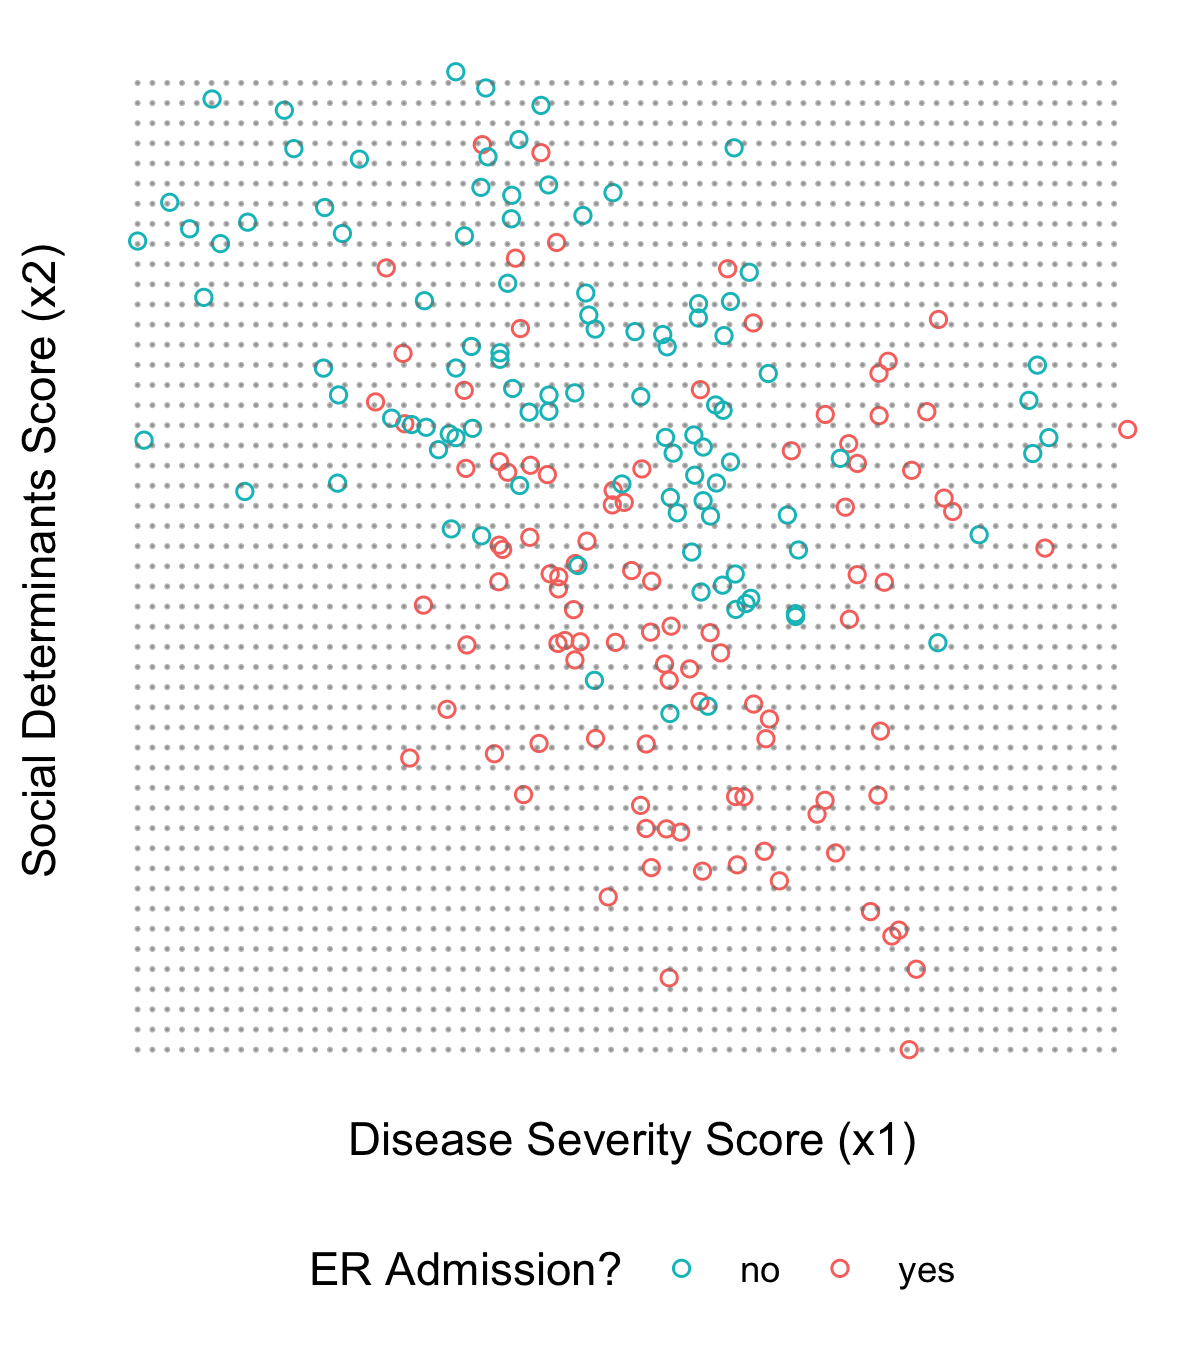
\includegraphics[width=0.7\textwidth]{img/esl-just-data.png}
\end{center}

Our goal in classification is to draw a \textbf{decision boundary}\index{decision boundary} through this space, on one side of which we will predict the patient to be readmitted, and on the other side of which we will predict the patient \emph{not} to be readmitted. The question in classification is: How do we draw a good boundary? How do we draw a boundary that will lead to accurate predictions on patients our model has never seen before?

%%%%%%%%%%%%%%%%%%%%%%%%%%%%%%%%%%%%%%%%%%%%%%%%%%%%%%%%%%%%%%%%%%%%%%%%%%%%%%%%%%%%%%

\section{Three Classification Algorithms}

\subsection{Logistic Regression}

The simplest decision boundary is, arguably, a line. The logistic regression\index{logistic regression} algorithm simply draws a line\footnote{In a higher-dimensional feature space, the decision boundary for logistic regression is a \textbf{hyperplane}.} through the feature space that divides the positive and negative training examples. 

\begin{center}
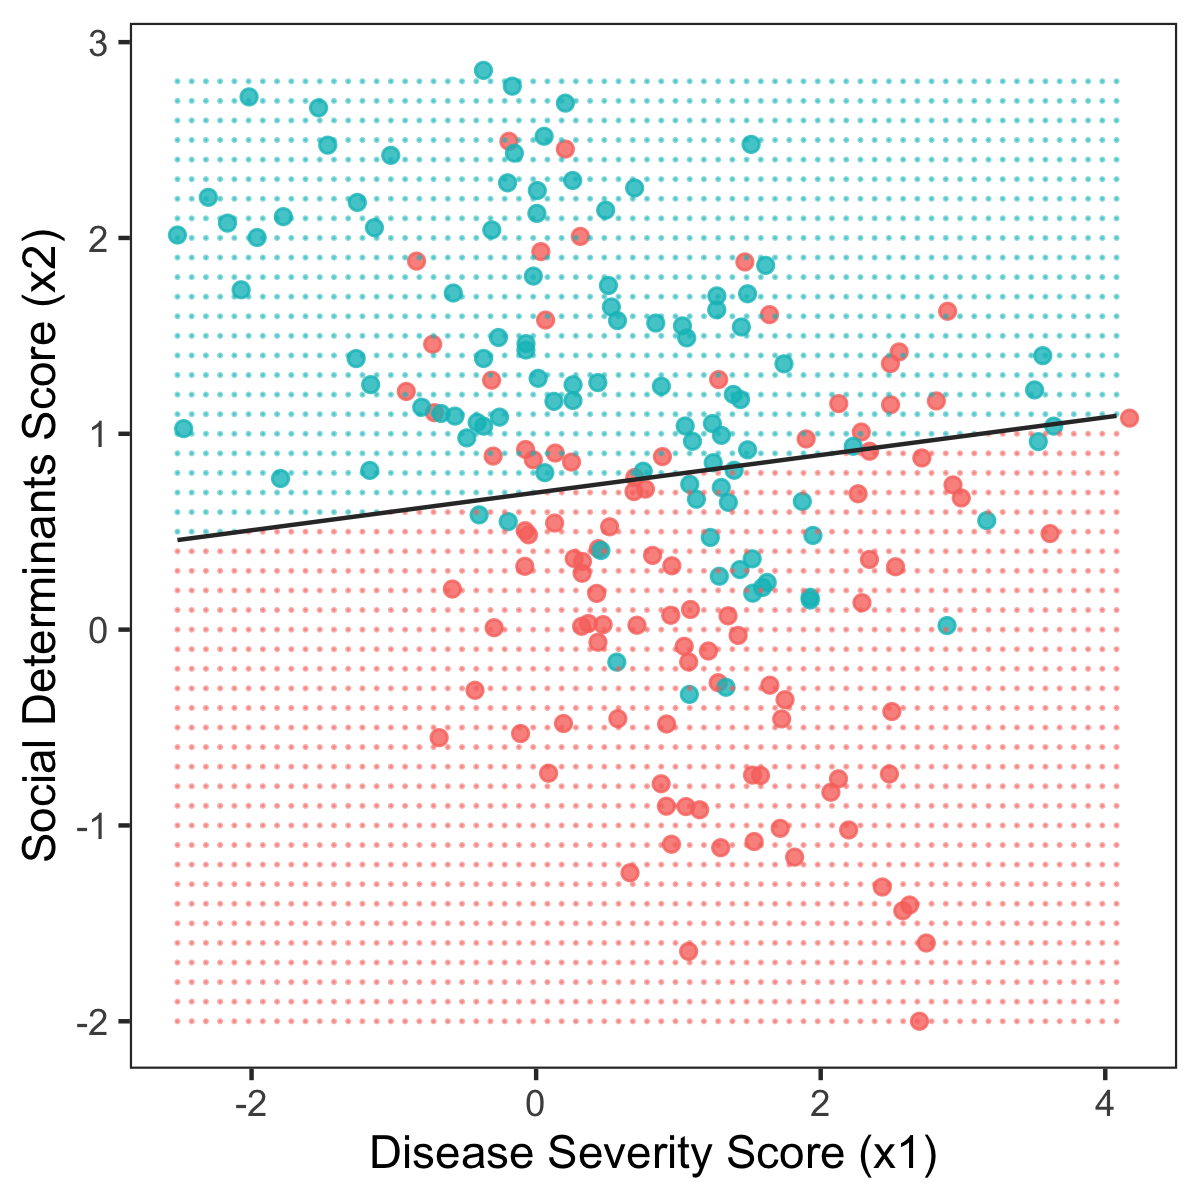
\includegraphics[width=0.7\textwidth]{img/esl-logistic.png}
\end{center}

\subsection{K Nearest Neighbors (KNN)}

Another approach is to make no assumptions about the shape of the decision boundary. To make a prediction about a new patient, we simply allow the $K$ nearest neighbors to vote. The parameter $K$ must be set independently and is called a \textbf{hyperparameter}. 

\noindent Here is the decision boundary for KNN with $K=15$:
\begin{center}
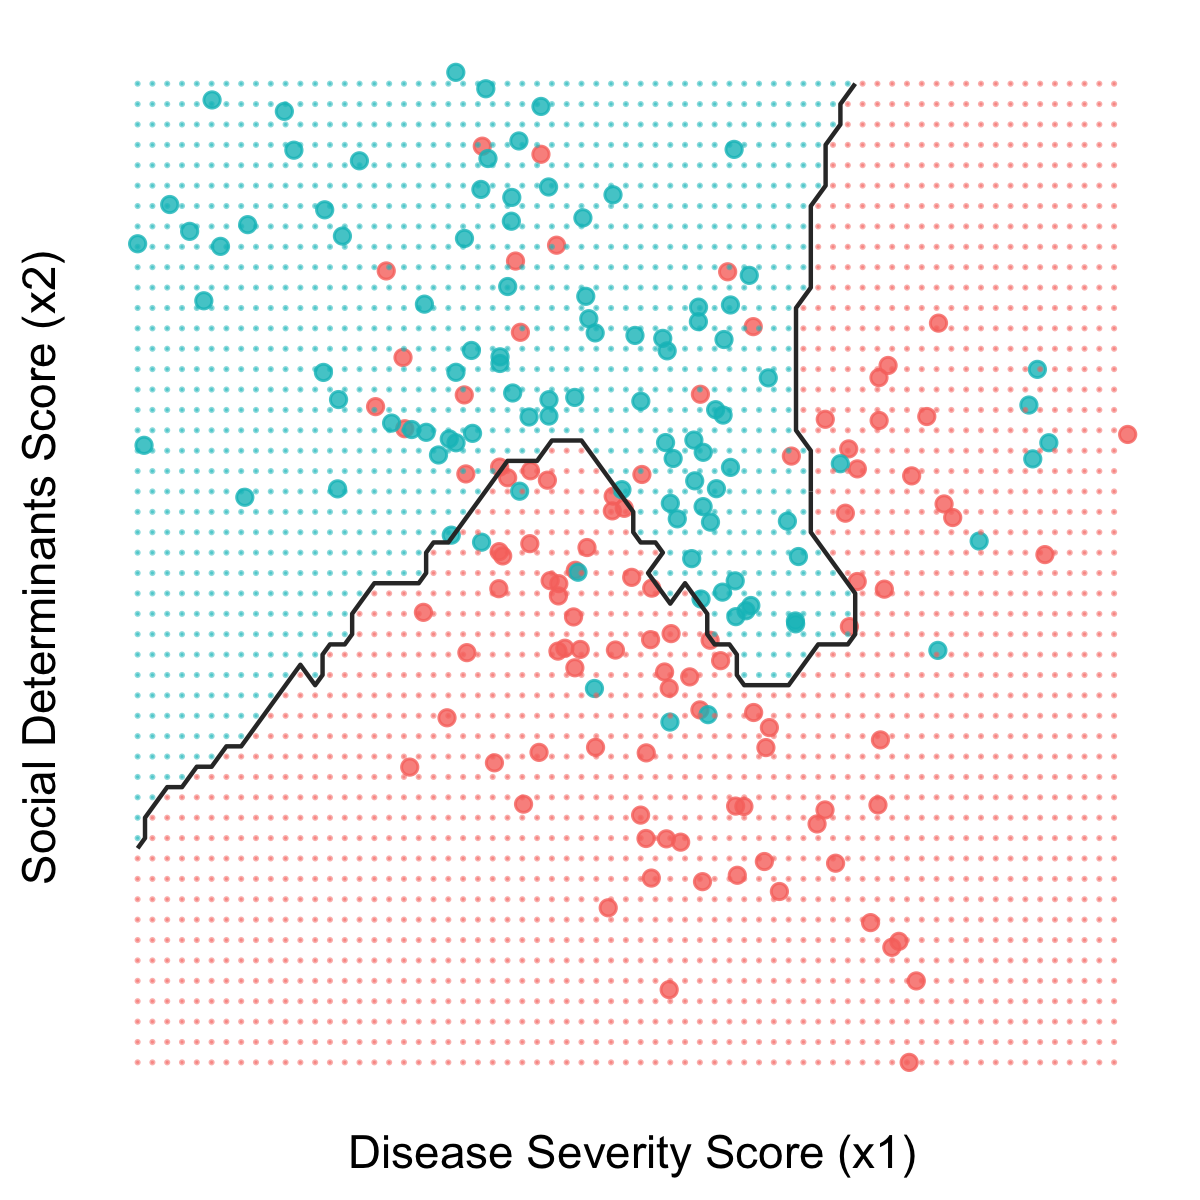
\includegraphics[width=0.7\textwidth]{img/esl-knn-15.png}
\end{center}

\subsection{Decision Tree}

Finally, we may choose to use our training data to build a decision tree\index{decision tree}, which will allow us to make predictions on new patients using a series of simple yes/no questions. There are different decision tree learning algorithms, but here is the tree produced by a famous one called CART:
\begin{center}
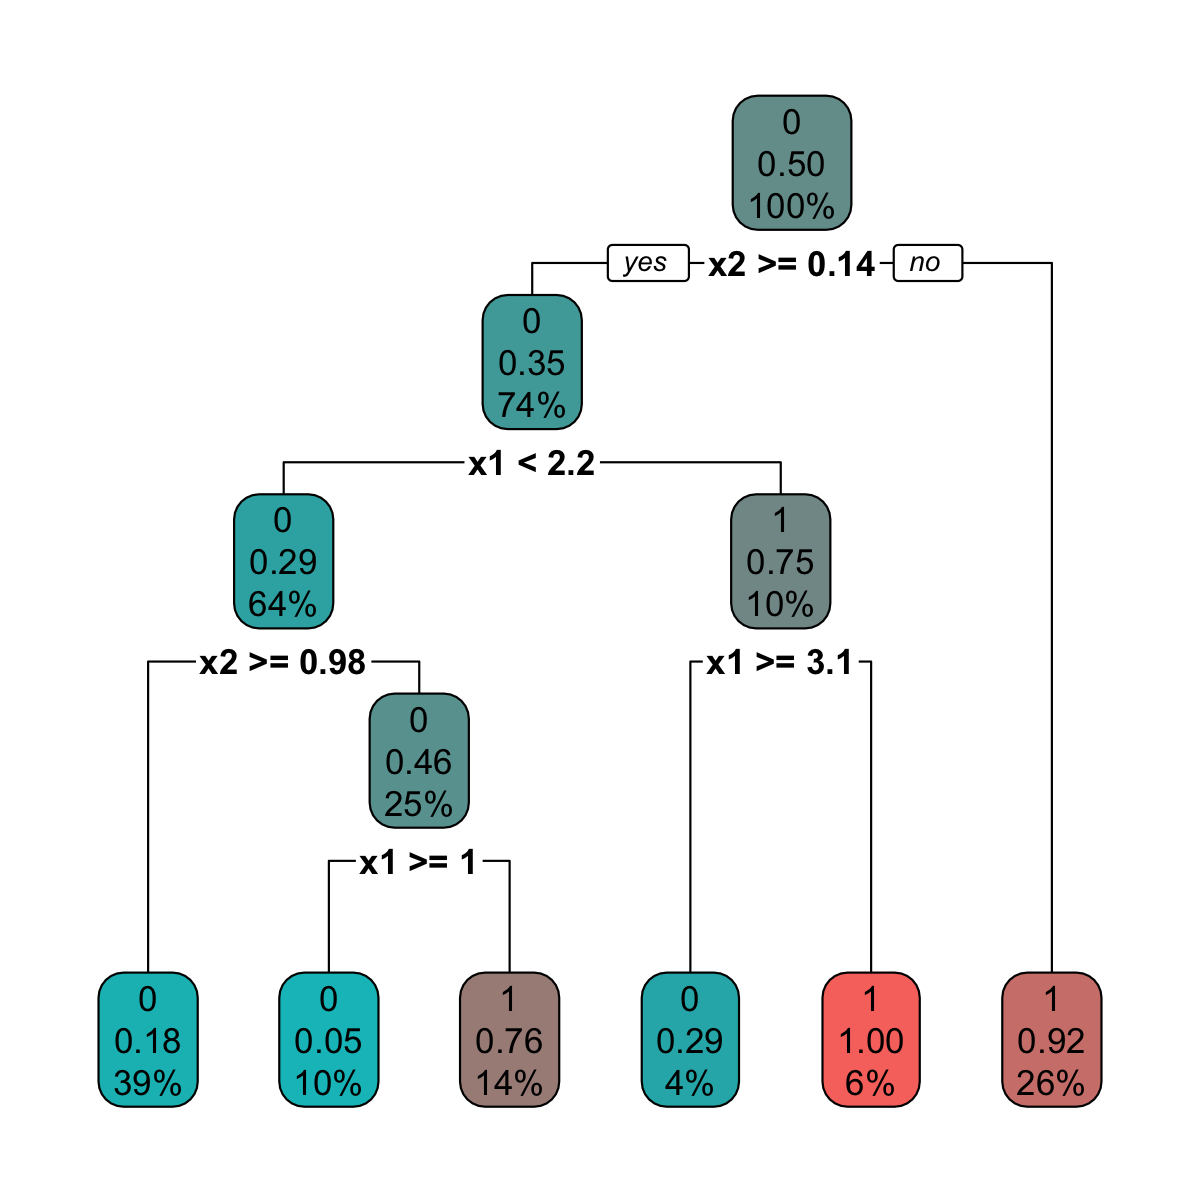
\includegraphics[width=0.6\textwidth]{img/esl-decision-tree-just-tree.png}
\end{center}
And here is the decision boundary produced by this tree:
\begin{center}
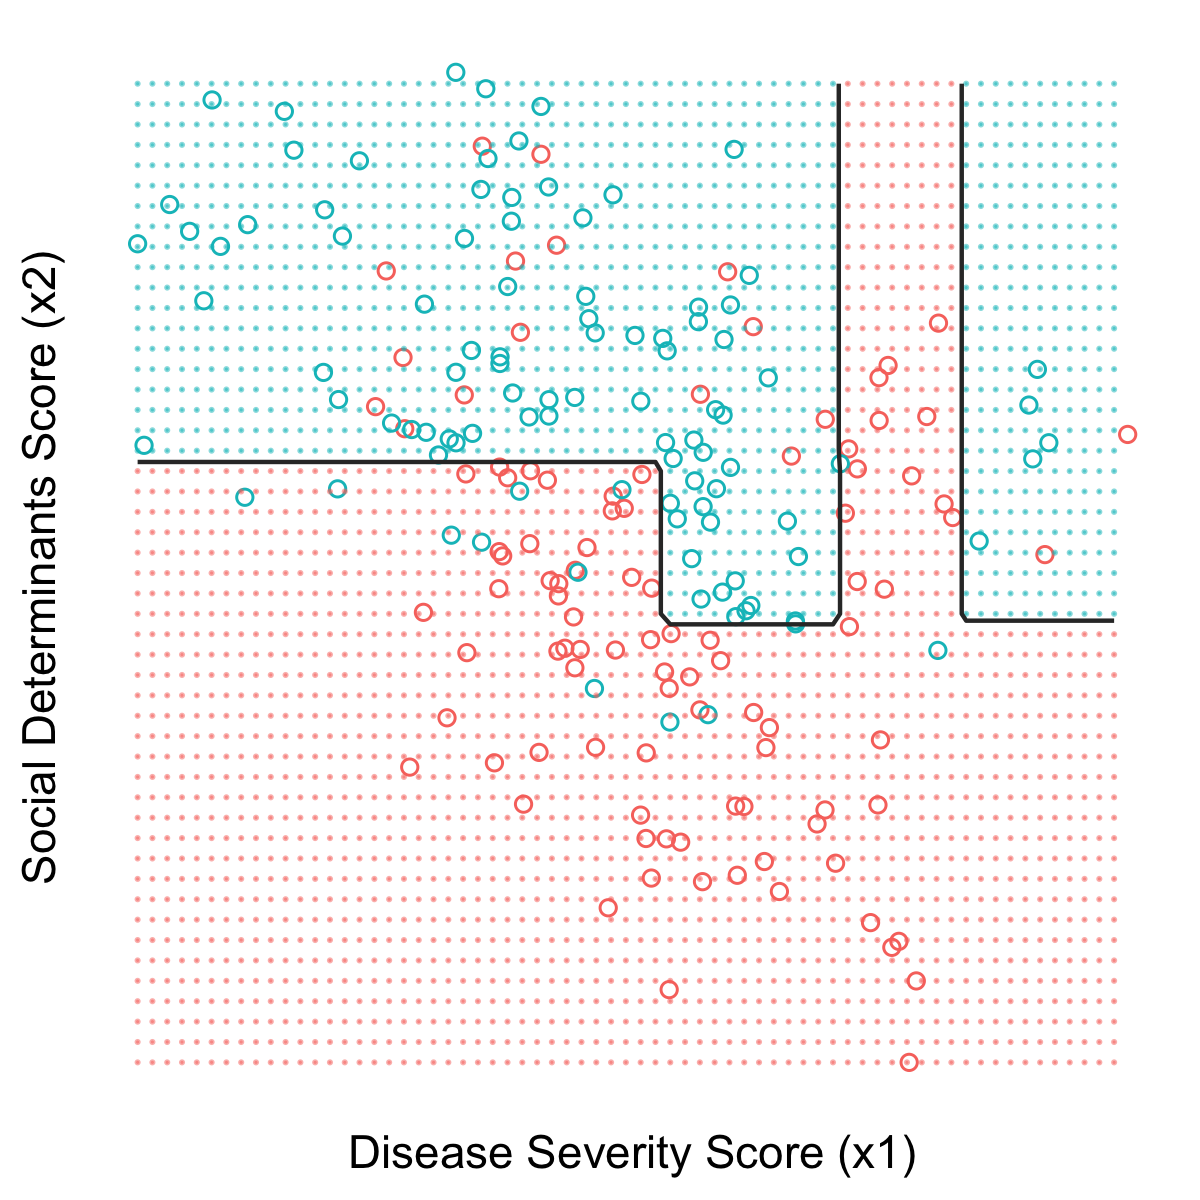
\includegraphics[width=0.7\textwidth]{img/esl-decision-tree.png}
\end{center}

\begin{question}{}
What are the advantages and disadvantages of the decision boundaries produced by:
  \begin{enumerate}
  \item Logistic regression?
  \item KNN ($K=15$)?
  \item Decision tree?
  \end{enumerate}
\end{question}

%%%%%%%%%%%%%%%%%%%%%%%%%%%%%%%%%%%%%%%%%%%%%%%%%%%%%%%%%%%%%%%%%%%%%%%%%%%%%%%%%%%%%%

\section{Classification with Probabilities}

We can think of classification as simply drawing a decision boundary, but underlying each algorithm is a quantitative assessment of each point in the feature space. Each algorithm is, in its own way, able to provide a degree of certainty, or \textbf{probability}\footnote{Pedantic footnote: this is a Bayesian definition of probability, as opposed to a frequentist definition. More on that later.}, that a point belongs to the positive outcome class. 

For example, here is the feature space of the example we just saw, colored by the probability, according to logistic regression, that a sample at each point should be classified as positive (i.e. the patient will be readmitted to the ER): 
\begin{center}
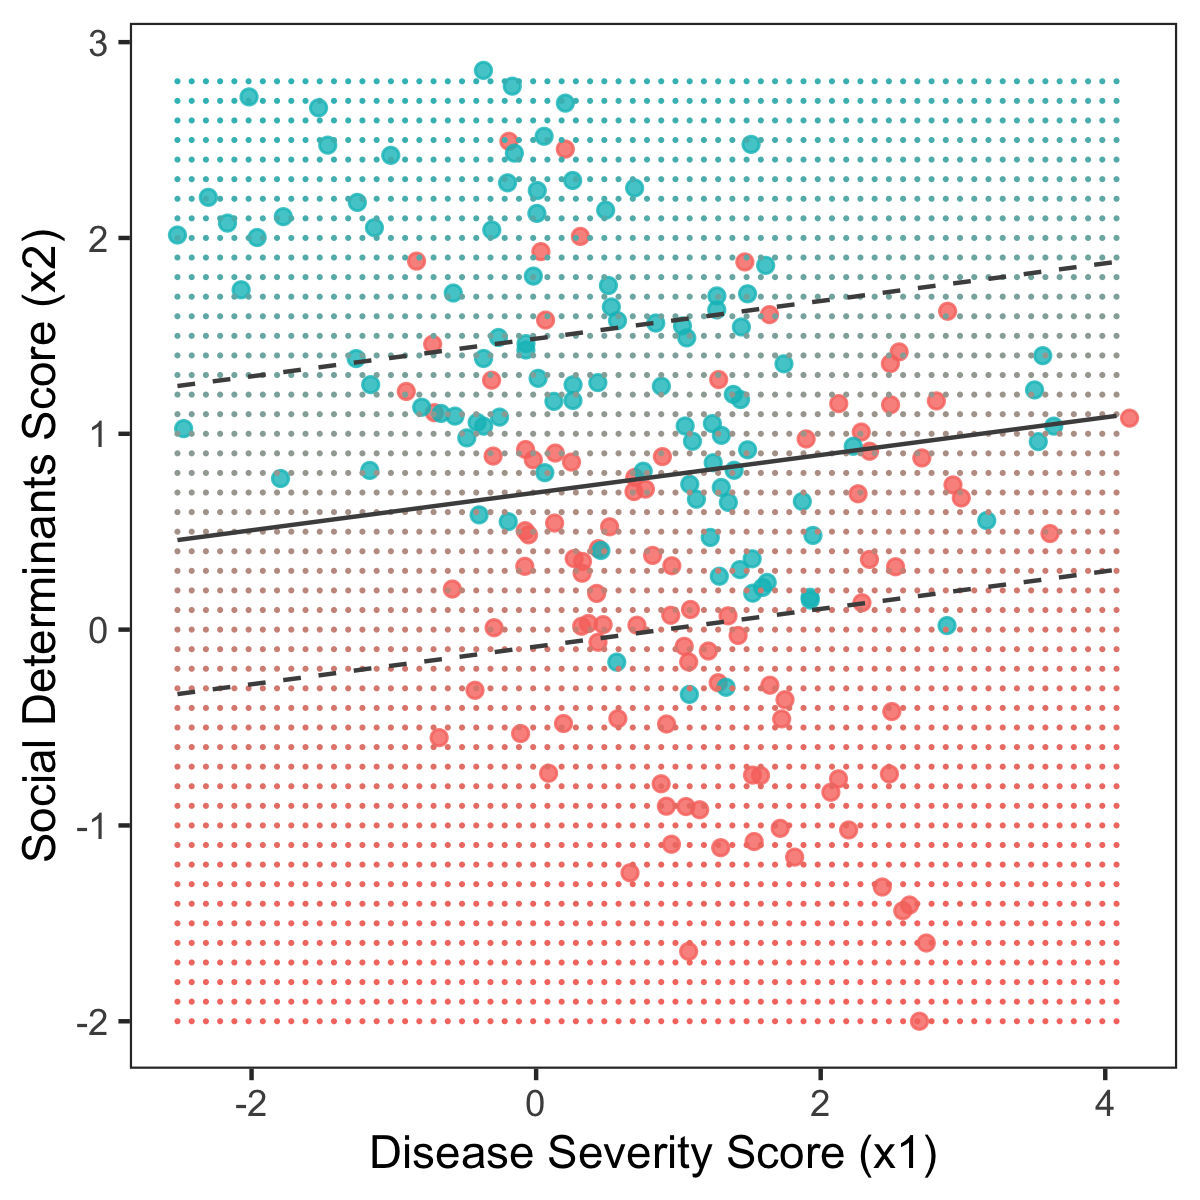
\includegraphics[width=0.7\textwidth]{img/esl-logistic-prob.png}
\end{center}

The solid line is the decision boundary, and the dashed lines indicate where the probability of a positive outcome (ER readmission) is 25\% (top line) and 75\% (bottom line). You can see that the color of the background gets purer red or purer blue the further you get from the decision boundary, but that near the decision boundary, the color is rather murky. That murkiness reflects the algorithm's uncertainty about the outcome. At the decision boundary, it is maximally uncertain. There the probability of a positive outcome is 50\%: a coin toss. 

\noindent Now, here is a similar plot for KNN ($K=15$): 
\begin{center}
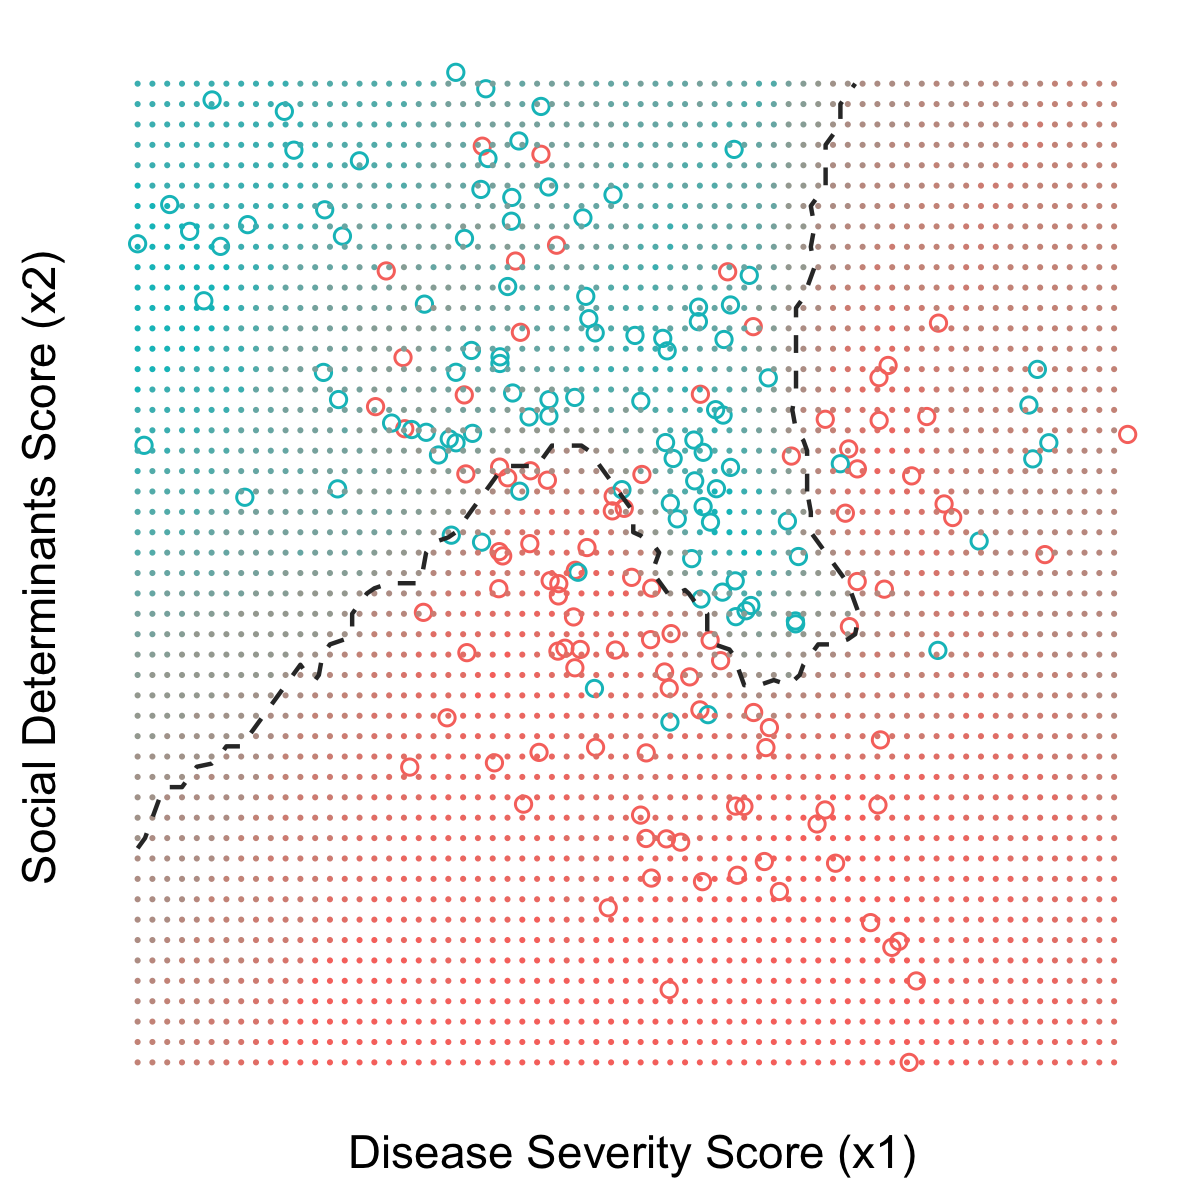
\includegraphics[width=0.68\textwidth]{img/esl-knn-15-prob.png}
\end{center}

You can see that the shapes of the 25\% and 75\% probability lines have much more complex shapes than for logistic regression, but the story is the same: you have regions of pure blue or red, where the algorithm is certain, and you have a murky region near the decision boundary. 

Finally, here is the same plot for the decision tree:
\begin{center}
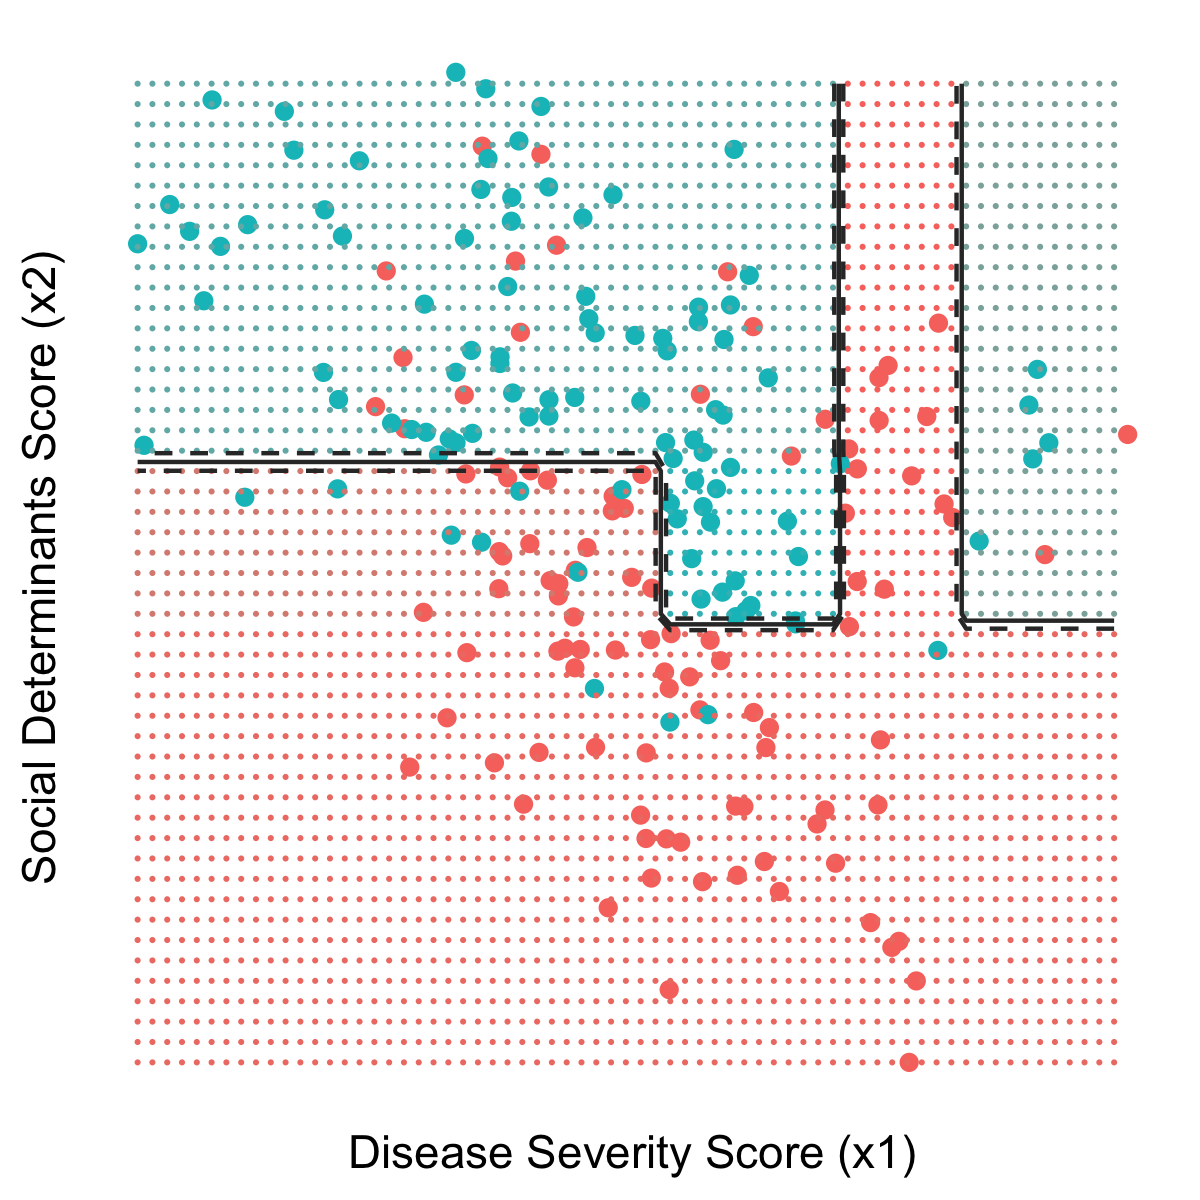
\includegraphics[width=0.68\textwidth]{img/esl-decision-tree-prob.png}
\end{center}
In this case, the color of the background in the different regions is relatively flat. The probability in each rectangular region (corresponding to each leaf of the tree) is constant. It equals the number of red dots in that region divided by the total number of dots. (Convince yourself of this.) 

\vspace{5mm}

\begin{question}{}
There are six rectangular regions in this picture corresponding to the six leaves of the tree. Identify all six and which leaves they correspond to on the decision tree, above.
\end{question}

\begin{question}{}
What makes a good classification algorithm? Consider issues of accuracy, generalizability, and speed (both to train the algorithm and to use it to make predictions on new samples). 
\end{question}

\begin{question}{}
The logistic regression, KNN, and decision tree algorithms can all be applied to address multi-outcome (i.e. more than two categories) classification problems with only minor modifications. Describe how each could be modified to work in these situations. (Think through this yourself before you Google.)
\end{question}

